% !TeX program = xelatex

\documentclass{beamer}

\usepackage[utf8]{inputenc}
\usepackage{graphicx}
\usepackage{listings}


% for table
\usepackage{bbding}
\usepackage{threeparttable,tabularx}
\usepackage{booktabs}
\newcommand{\yes}{\textcolor{green}{\CheckmarkBold}}
\newcommand{\no}{\textcolor{red}{\XSolidBrush}}

%Tamarin Code Highlighter
\definecolor{dartmouthgreen}{rgb}{0.05, 0.5, 0.06}
\lstdefinelanguage{Tamarin}{
	alsoletter={-},
	keywords=[1]{},
	otherkeywords={[, ], --, ->, [, \t\,},
	keywords=[2]{let, in, exists-trace},
	keywords=[3]{rule, lemma, Ex, All, not},
	keywords=[4]{RevDHQ},
	keywordstyle=[1]{\color{black}\bfseries},
	keywordstyle=[2]{\color{dartmouthgreen}\bfseries},
	keywordstyle=[3]{\color{blue}\bfseries},
	keywordstyle=[4]{\color{magenta}\itshape\bfseries},
	string=[b]{'},
	stringstyle=\color{red},
	numbers=left,
	numberstyle=\scriptsize,
	stepnumber=1,
	numbersep=8pt,
	comment=[l]{//},
	morecomment=[s]{/*}{*/},
	commentstyle=\color{gray!75},
	basicstyle=\normalfont\ttfamily,
	breakatwhitespace=false,         % sets if automatic breaks should only happen at whitespace
	breaklines=true,                 % sets automatic line breaking
	captionpos=b                    % sets the caption-position to bottom
}


\lstset{
  frame=single,
  basicstyle=\footnotesize\ttfamily,
  captionpos=b,
  tabsize=2,
}
\beamertemplatenavigationsymbolsempty
\setbeamertemplate{footline}{%
\insertframenumber{}/\inserttotalframenumber}


%Information to be included in the title page:
\title{A formal analysis of IKEv2's post-quantum extension}
\usecolortheme{dove}
\author{Stefan-Lukas Gazdag, Sophia Grundner-Culemann,\\
    Tobias Guggemos, \underline{Tobias Heider},\\
    Daniel Loebenberger}
\institute{ACSAC2021}
\date{12/08/21}

\setbeamertemplate{itemize items}[circle]
\setbeamertemplate{itemize subitem}[default] \begin{document}

\begin{frame}[noframenumbering, plain]
	\titlepage
\end{frame}

\begin{frame}
\frametitle{The IKEv2 Protocol}
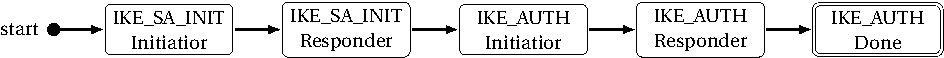
\includegraphics[width=\textwidth]{ike-state-machine.pdf}
\end{frame}

\begin{frame}
\frametitle{Post-Quantum IKEv2}
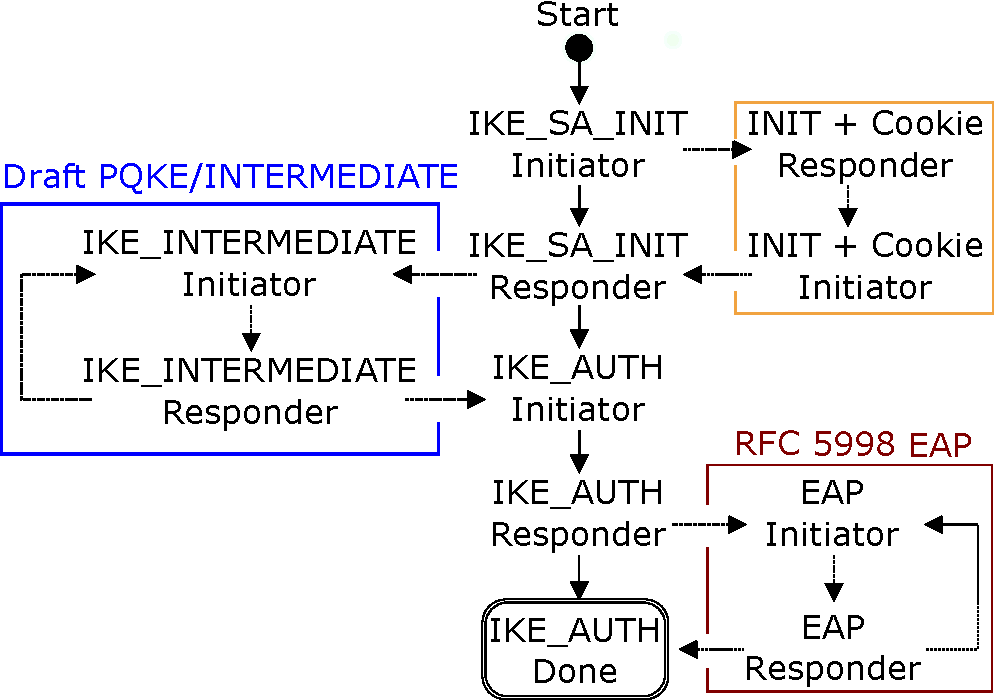
\includegraphics[width=\textwidth]{statemachine.pdf}
\end{frame}

\begin{frame}
\frametitle{The Tamarin Prover}
$\underline{\text{Idea:}}$  
\begin{itemize}
	\item symbolic analysis
	\item transition system
	\begin{itemize}
		\item ``exists-trace'' 
		\item ``all traces fulfill ... '' 
	\end{itemize}
\end{itemize}
\end{frame}

\begin{frame}[fragile]
\frametitle{The Tamarin Prover}
\begin{lstlisting}[language=Tamarin]
rule reveal_dh:
[ !DHtoReveal($I, k) ] 
--[RevDH($I)]->       
[ Out(k) ]   
\end{lstlisting}
\end{frame}

\begin{frame}
\frametitle{IKEv2 Security Model}
\begin{itemize}
	\item Dolev-Yao attacker
\end{itemize}
\pause
\bigskip
$\underline{\text{Security properties:}}$              
\pause
\begin{itemize}	
	\item Consistency
	\pause
	\item Key secrecy
	\pause
	\item Identity Protection
	\pause
	\item Agreement: \smallskip
	\pause
	\begin{itemize}
		\item Aliveness \textit{of Initiator and of Responder} 
		\pause        
		\item Weak Agreement \textit{of I. and of R.}
		\pause
		\item Agreement\textit{ of I. and of R.}		
	\end{itemize}
	
\end{itemize}
\end{frame}

\begin{frame}
	\frametitle{Modeling PQ-IKEv2}
	
\end{frame}

\begin{frame}
\frametitle{Result}
\begin{table}[t]
\resizebox{.7\textwidth}{!}{
	\begin{tabular}{m{1.6cm}ccccc}
		\toprule
		& none & I eph. & R eph. & I static & R static \\
		\midrule
		Aliveness\_I  & \yes &  \yes  &  \yes  &   \yes   &   \no    \\
		Aliveness\_R  & \yes &  \yes  &  \yes  &   \yes   &   \no    \\
		\uchyph=0 Weak Agreement\_I & \yes &  \no   &  \no   &   \yes   &   \no \\
		\uchyph=0 Weak Agreement\_R & \no &  \no   &  \no   &   \no   &   \no \\
		Agreement\_I & \yes &  \no   &  \no   &   \yes   &   \no    \\
		Agreement\_R & \no &  \no   &  \no   &   \no   &   \no    \\
		Consistency   & \yes &  \yes  &  \yes  &   \yes   &   \no    \\
		Key secrecy   & \yes &  \no   &  \no   &   \yes   &   \no    \\
		\uchyph=0 Identity Protection  & \yes &  \no   &  \no   &   \no    &   \yes \\
		\bottomrule
	\end{tabular}
}
\caption[]{\textbf{Implications of key compromise:} Each entry indicates whether the security property of the corresponding row is achieved (\yes{}) or not (\no{}) if the key of the corresponding column is compromised. } 
\end{table}
\end{frame}

\end{document}
